
% This LaTeX was auto-generated from an M-file by MATLAB.
% To make changes, update the M-file and republish this document.

\documentclass{article}
\usepackage[utf8]{inputenc}
\usepackage{graphicx}
\usepackage{epstopdf}
\usepackage{color}
\usepackage{xcolor}
\usepackage[ocgcolorlinks]{hyperref}
\usepackage{bookmark}
\usepackage[hmargin=2cm,vmargin=2.5cm]{geometry}
\usepackage{fancyhdr}

\sloppy
\definecolor{lightgray}{gray}{0.5}
\setlength{\parindent}{0pt}

\makeindex

\begin{document}

    
    
\tableofcontents
\newpage


\subsection*{Midterm PREP Script}
\addcontentsline{toc}{subsection}{Midterm PREP Script}
\phantomsection


        \begin{par}
Chapter 6 --- Stabability Question 1, Nise Textbook
\end{par} \vspace{1em}
\begin{verbatim}
clear all
close all
\end{verbatim}
\begin{par}
s\^{}5 +3s\^{}4+5s\^{}3 + 4s\^{}2+s+3
\end{par} \vspace{1em}
\begin{verbatim}
polyVector = [1 3 5 4 1 3]
RouthHurwitz(polyVector)
\end{verbatim}

        \color{lightgray} \begin{verbatim}
polyVector =

     1     3     5     4     1     3


 Routh-Hurwitz Table:

rhTable =

    1.0000    5.0000    1.0000
    3.0000    4.0000    3.0000
    3.6667         0         0
    4.0000    3.0000         0
   -2.7500         0         0
    3.0000         0         0

~~~~~> it is an unstable system! <~~~~~

 Number of right hand side poles = 2

 Given polynomial coefficients roots :

sysRoots =

  -1.6313 + 0.0000i
  -0.9407 + 1.5042i
  -0.9407 - 1.5042i
   0.2563 + 0.7201i
   0.2563 - 0.7201i


ans =

    1.0000    5.0000    1.0000
    3.0000    4.0000    3.0000
    3.6667         0         0
    4.0000    3.0000         0
   -2.7500         0         0
    3.0000         0         0

\end{verbatim} \color{black}
    \begin{par}
Q2
\end{par} \vspace{1em}
\begin{verbatim}
v2 = [1 0 6 5 8 20]
RouthHurwitz(v2)
\end{verbatim}

        \color{lightgray} \begin{verbatim}
v2 =

     1     0     6     5     8    20


 Routh-Hurwitz Table:

rhTable =

     1     6     8
     0     5    20
  -Inf  -Inf     0
   NaN   NaN     0
   NaN   NaN     0
   NaN   NaN     0

~~~~~> it is a stable system! <~~~~~

 Number of right hand side poles = 0

 Given polynomial coefficients roots :

sysRoots =

   0.6641 + 1.8230i
   0.6641 - 1.8230i
  -0.0000 + 2.0000i
  -0.0000 - 2.0000i
  -1.3283 + 0.0000i


ans =

     1     6     8
     0     5    20
  -Inf  -Inf     0
   NaN   NaN     0
   NaN   NaN     0
   NaN   NaN     0

\end{verbatim} \color{black}
    \begin{verbatim}
syms s
(s+1)*(s+2)*(s+3)*(s+4)
\end{verbatim}

        \color{lightgray} \begin{verbatim} 
ans =
 
(s + 1)*(s + 2)*(s + 3)*(s + 4)
 
\end{verbatim} \color{black}
    \begin{par}
syms a b c EPS;
\end{par} \vspace{1em}
\begin{verbatim}
syms a b c EPS;
ra=routh([1 a b c],EPS)
\end{verbatim}

        \color{lightgray} \begin{verbatim} 
ra =
 
[            1, b]
[            a, c]
[ -(c - a*b)/a, 0]
[            c, 0]
 
\end{verbatim} \color{black}
    

\subsection*{Question 12}
\addcontentsline{toc}{subsection}{Question 12}
\phantomsection


        \begin{par}
K(s+2)/s(s-1)(s+3)
\end{par} \vspace{1em}
\begin{verbatim}
syms s K EPS;
ra2 = routh([1 2 K-3 2],EPS)
\end{verbatim}

        \color{lightgray} \begin{verbatim} 
ra2 =
 
[                 1, K - 3]
[                 2,     2]
[             K - 4,     0]
[ (2*K - 8)/(K - 4),     0]
 
\end{verbatim} \color{black}
    

\subsection*{Quesition 20}
\addcontentsline{toc}{subsection}{Quesition 20}
\phantomsection


        \begin{verbatim}
ra3 = routh([K+1 3 2+K],EPS)
\end{verbatim}

        \color{lightgray} \begin{verbatim} 
ra3 =
 
[ K + 1, K + 2]
[     3,     0]
[ K + 2,     0]
 
\end{verbatim} \color{black}
    

\subsection*{Question 21}
\addcontentsline{toc}{subsection}{Question 21}
\phantomsection


        \begin{verbatim}
ra4 = routh([1 5 4+K 6*K],EPS)
% solve(4 - K/5==0)
% solve((6*K*(K - 20))/(5*(K/5 - 4))==0)
\end{verbatim}

        \color{lightgray} \begin{verbatim} 
ra4 =
 
[                            1, K + 4]
[                            5,   6*K]
[                      4 - K/5,     0]
[ (6*K*(K - 20))/(5*(K/5 - 4)),     0]
 
\end{verbatim} \color{black}
    

\subsection*{Question 22}
\addcontentsline{toc}{subsection}{Question 22}
\phantomsection


        \begin{verbatim}
syms a b c EPS;
ra5 = routh([1 K-b -a],EPS)
\end{verbatim}

        \color{lightgray} \begin{verbatim} 
ra5 =
 
[     1, -a]
[ K - b,  0]
[    -a,  0]
 
\end{verbatim} \color{black}
    

\subsection*{Example 7.2 from Nise}
\addcontentsline{toc}{subsection}{Example 7.2 from Nise}
\phantomsection


        \begin{verbatim}
syms s
Gs = 120*(s+2)/((s+3)*(s+4))
CSlashR = simplify(Gs/(1+Gs))
polyVector = [1 127 252]
routh([1 127 252],EPS)
limit(Gs,s,0)
limit(s*Gs,s,0)

limit(s^2*Gs,s,0)
\end{verbatim}

        \color{lightgray} \begin{verbatim} 
Gs =
 
(120*s + 240)/((s + 3)*(s + 4))
 
 
CSlashR =
 
(120*s + 240)/(s^2 + 127*s + 252)
 

polyVector =

     1   127   252

 
ans =
 
[   1, 252]
[ 127,   0]
[ 252,   0]
 
 
ans =
 
20
 
 
ans =
 
0
 
 
ans =
 
0
 
\end{verbatim} \color{black}
    

\subsection*{Example 7.3 from Nise}
\addcontentsline{toc}{subsection}{Example 7.3 from Nise}
\phantomsection


        \begin{verbatim}
syms s
Gs =100*(s+2)*(s+6)/(s*(s+3)*(s+4))
CSlashR = simplify(Gs/(1+Gs))
polyVector = [1 107 812 1200]
routh(polyVector, EPS)
%R(s) = 5*1/s
limit(5/(1+Gs),s,0)
\end{verbatim}

        \color{lightgray} \begin{verbatim} 
Gs =
 
((100*s + 200)*(s + 6))/(s*(s + 3)*(s + 4))
 
 
CSlashR =
 
(100*s^2 + 800*s + 1200)/(s^3 + 107*s^2 + 812*s + 1200)
 

polyVector =

           1         107         812        1200

 
ans =
 
[         1,  812]
[       107, 1200]
[ 85684/107,    0]
[      1200,    0]
 
 
ans =
 
0
 
\end{verbatim} \color{black}
    

\subsection*{Example 7.4 from Nise}
\addcontentsline{toc}{subsection}{Example 7.4 from Nise}
\phantomsection


        \begin{verbatim}
Gs = 10*(s+20)*(s+30)/((s*(s+25)*(s+35)))
CSlashR = simplify(Gs/(1+Gs))
polyVector = [1 70 1375 600]
routh(polyVector, EPS)
\end{verbatim}

        \color{lightgray} \begin{verbatim} 
Gs =
 
((10*s + 200)*(s + 30))/(s*(s + 25)*(s + 35))
 
 
CSlashR =
 
(10*s^2 + 500*s + 6000)/(s^3 + 70*s^2 + 1375*s + 6000)
 

polyVector =

           1          70        1375         600

 
ans =
 
[      1, 1375]
[     70,  600]
[ 9565/7,    0]
[    600,    0]
 
\end{verbatim} \color{black}
    \begin{verbatim}
Gs = 10*(s+20)*(s+30)/((s^2*(s+25)*(s+35)*(s+50)))
CSlashR = simplify(Gs/(1+Gs))
polyVector = [1 110 3875 43760 500 6000]
routh(polyVector, EPS)
\end{verbatim}

        \color{lightgray} \begin{verbatim} 
Gs =
 
((10*s + 200)*(s + 30))/(s^2*(s + 25)*(s + 35)*(s + 50))
 
 
CSlashR =
 
(10*s^2 + 500*s + 6000)/(s^5 + 110*s^4 + 3875*s^3 + 43760*s^2 + 500*s + 6000)
 

polyVector =

           1         110        3875       43760         500        6000

 
ans =
 
[                    1,    3875,  500]
[                  110,   43760, 6000]
[             38249/11, 4900/11,    0]
[     1673237240/38249,    6000,    0]
[ -1316030750/41830931,       0,    0]
[                 6000,       0,    0]
 
\end{verbatim} \color{black}
    \begin{verbatim}
G1(s) = 500*(s+2)*(s+5)/((s+8)*(s+10)*(s+12))
G2(s) = 500*(s+5)*(s+5)*(s+6)/(s*(s+8)*(s+10)*(s+12))
G3(s) = 500*(s+2)*(s+4)*(s+5)*(s+6)*(s+7)/(s^2*(s+8)*(s+10)*(s+12))
Func1 = (simplify(G1(s)/(1+G1(s))))
Func2 = (simplify(G2(s)/(1+G2(s))))
Func3 = (simplify(G3(s)/(1+G3(s))))
\end{verbatim}

        \color{lightgray} \begin{verbatim} 
G1(s) =
 
((500*s + 1000)*(s + 5))/((s + 8)*(s + 10)*(s + 12))
 
 
G2(s) =
 
((500*s + 2500)*(s + 5)*(s + 6))/(s*(s + 8)*(s + 10)*(s + 12))
 
 
G3(s) =
 
((500*s + 1000)*(s + 4)*(s + 5)*(s + 6)*(s + 7))/(s^2*(s + 8)*(s + 10)*(s + 12))
 
 
Func1 =
 
(500*s^2 + 3500*s + 5000)/(s^3 + 530*s^2 + 3796*s + 5960)
 
 
Func2 =
 
(500*(s + 5)^2*(s + 6))/(s^4 + 530*s^3 + 8296*s^2 + 43460*s + 75000)
 
 
Func3 =
 
(500*s^5 + 12000*s^4 + 111500*s^3 + 498000*s^2 + 1058000*s + 840000)/(501*s^5 + 12030*s^4 + 111796*s^3 + 498960*s^2 + 1058000*s + 840000)
 
\end{verbatim} \color{black}
    \begin{verbatim}
[n1,d1] = numden(Func1)
routh(sym2poly(d1), EPS)
[n2,d2] = numden(Func2)
routh(sym2poly(d2), EPS)
[n3,d3] = numden(Func3)
routh(sym2poly(d3), EPS)

Kp = limit(G1(s),s,0)
Kv = limit(s*G2(s),s,0)
Ka = limit(s^2*G3(s),s,0)
\end{verbatim}

        \color{lightgray} \begin{verbatim} 
n1 =
 
500*s^2 + 3500*s + 5000
 
 
d1 =
 
s^3 + 530*s^2 + 3796*s + 5960
 
 
ans =
 
[         1, 3796]
[       530, 5960]
[ 200592/53,    0]
[      5960,    0]
 
 
n2 =
 
500*(s + 5)^2*(s + 6)
 
 
d2 =
 
s^4 + 530*s^3 + 8296*s^2 + 43460*s + 75000
 
 
ans =
 
[             1,  8296, 75000]
[           530, 43460,     0]
[          8214, 75000,     0]
[ 52871740/1369,     0,     0]
[         75000,     0,     0]
 
 
n3 =
 
500*s^5 + 12000*s^4 + 111500*s^3 + 498000*s^2 + 1058000*s + 840000
 
 
d3 =
 
501*s^5 + 12030*s^4 + 111796*s^3 + 498960*s^2 + 1058000*s + 840000
 
 
ans =
 
[                           501,        111796, 1058000]
[                         12030,        498960,  840000]
[                  36497564/401, 410230000/401,       0]
[         3318939408360/9124391,        840000,       0]
[ 22481158689222000/27657828403,             0,       0]
[                        840000,             0,       0]
 
 
Kp =
 
125/24
 
 
Kv =
 
625/8
 
 
Ka =
 
875
 
\end{verbatim} \color{black}
    \begin{par}
Try
\end{par} \vspace{1em}
\begin{verbatim}
numg=1000*[1 8];
deng=poly([-7 -9]);
G=tf(numg,deng);
Kp=dcgain(G)
estep=1/(1+Kp)
T=feedback(G,1);
poles=pole(T)
\end{verbatim}

        \color{lightgray} \begin{verbatim}
Kp =

  126.9841


estep =

    0.0078


poles =

   1.0e+03 *

   -1.0080
   -0.0080

\end{verbatim} \color{black}
    

\subsection*{Chapter 7 or 8 root Locus Plots}
\addcontentsline{toc}{subsection}{Chapter 7 or 8 root Locus Plots}
\phantomsection


        \begin{par}
Root Locus Plot
\end{par} \vspace{1em}
\begin{verbatim}
h = tf([2 5 1],[1 2 3]);
rlocus(h)
snapnow;
\end{verbatim}

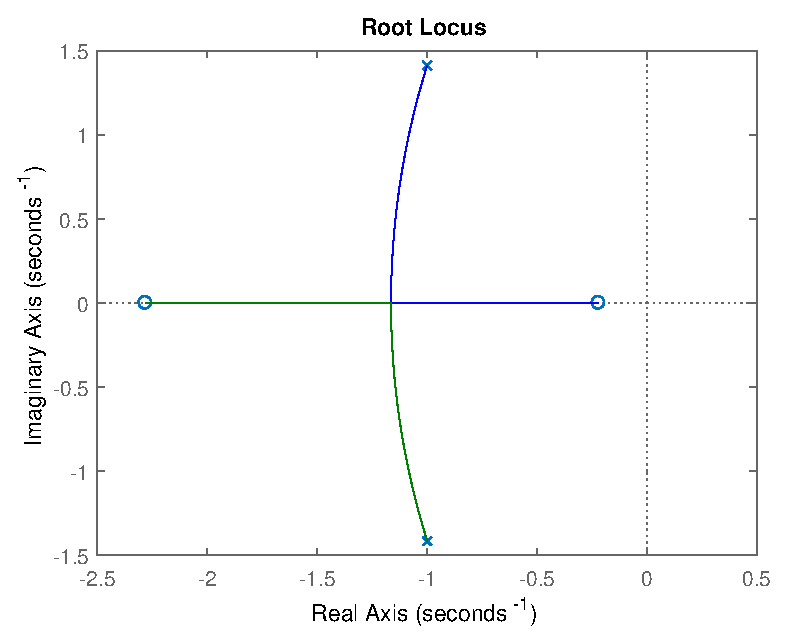
\includegraphics [width=7in]{MidtermPrep_01.eps}
\begin{par}
Example from textbook
\end{par} \vspace{1em}
\begin{verbatim}
syms s
x = s*(s+1)*(s+2)*(s+4)
den = sym2poly(x)
num = (s+3)
num = sym2poly(num)
h = tf([num],[den])
rlocus(h)
\end{verbatim}

        \color{lightgray} \begin{verbatim} 
x =
 
s*(s + 1)*(s + 2)*(s + 4)
 

den =

     1     7    14     8     0

 
num =
 
s + 3
 

num =

     1     3


h =
 
            s + 3
  --------------------------
  s^4 + 7 s^3 + 14 s^2 + 8 s
 
Continuous-time transfer function.

\end{verbatim} \color{black}
    
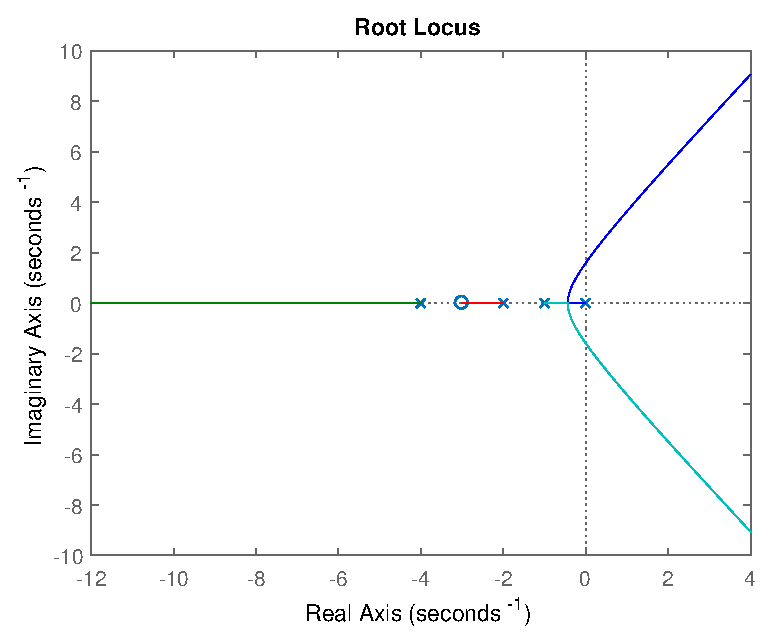
\includegraphics [width=7in]{MidtermPrep_02.eps}
\begin{par}
$$ $$
\end{par} \vspace{1em}
\begin{verbatim}
x = (s+2)*(s+4)*(s+6)
den = sym2poly(x)
h = tf([1],[den])
rlocus(h)
\end{verbatim}

        \color{lightgray} \begin{verbatim} 
x =
 
(s + 2)*(s + 4)*(s + 6)
 

den =

     1    12    44    48


h =
 
             1
  ------------------------
  s^3 + 12 s^2 + 44 s + 48
 
Continuous-time transfer function.

\end{verbatim} \color{black}
    
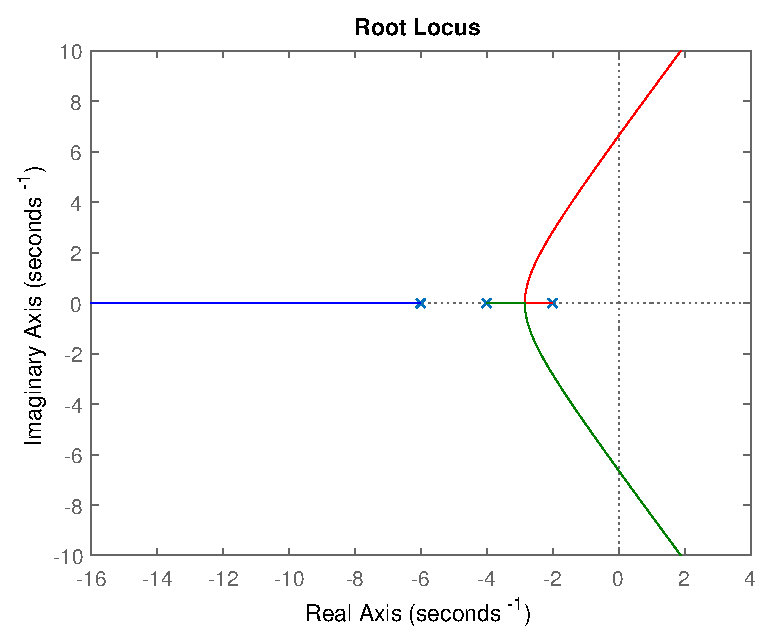
\includegraphics [width=7in]{MidtermPrep_03.eps}
\begin{verbatim}
syms s K EPS
x =s^4+ 7*s^3+14*s^2+(8+K)*s+3*K
polyVec = [1 7 14 8+K 3*K]
xD = routh(polyVec, EPS)
xD = simplify(xD)
\end{verbatim}

        \color{lightgray} \begin{verbatim} 
x =
 
s^4 + 7*s^3 + 14*s^2 + (K + 8)*s + 3*K
 
 
polyVec =
 
[ 1, 7, 14, K + 8, 3*K]
 
 
xD =
 
[                                                                           1,    14, 3*K]
[                                                                           7, K + 8,   0]
[                                                                  90/7 - K/7,   3*K,   0]
[                                     (K^2/7 + (65*K)/7 - 720/7)/(K/7 - 90/7),     0,   0]
[ (3*K*(K/7 - 90/7)*(K^2 + 65*K - 720))/((K - 90)*(K^2/7 + (65*K)/7 - 720/7)),     0,   0]
 
 
xD =
 
[                           1,    14, 3*K]
[                           7, K + 8,   0]
[                  90/7 - K/7,   3*K,   0]
[ (K^2 + 65*K - 720)/(K - 90),     0,   0]
[                         3*K,     0,   0]
 
\end{verbatim} \color{black}
    \begin{verbatim}
polyVec = [1 6 8]
routh(polyVec,EPS)
% stable function
rlocus(tf([1 4 20],[1 6 8]))
\end{verbatim}

        \color{lightgray} \begin{verbatim}
polyVec =

     1     6     8

 
ans =
 
[ 1, 8]
[ 6, 0]
[ 8, 0]
 
\end{verbatim} \color{black}
    
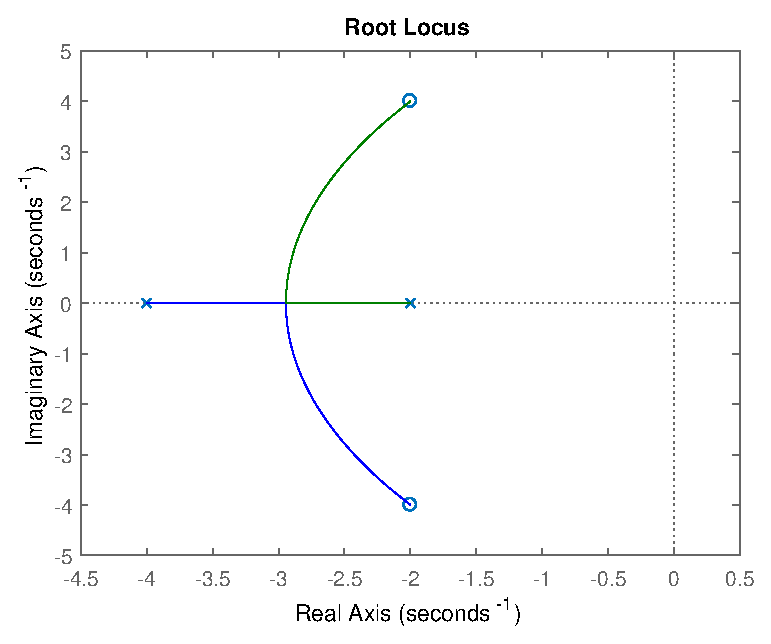
\includegraphics [width=7in]{MidtermPrep_04.eps}
\begin{par}
Question 8--4
\end{par} \vspace{1em}
\begin{verbatim}
num= tf([1 2/3])
den = tf([1 6 0 0])

sys = tf([1 2/3], [1 6 0 0])
rlocus(sys)
\end{verbatim}

        \color{lightgray} \begin{verbatim}
num =
 
  From input 1 to output:
  1
 
  From input 2 to output:
  0.6667
 
Static gain.


den =
 
  From input 1 to output:
  1
 
  From input 2 to output:
  6
 
  From input 3 to output:
  0
 
  From input 4 to output:
  0
 
Static gain.


sys =
 
  s + 0.6667
  -----------
  s^3 + 6 s^2
 
Continuous-time transfer function.

\end{verbatim} \color{black}
    
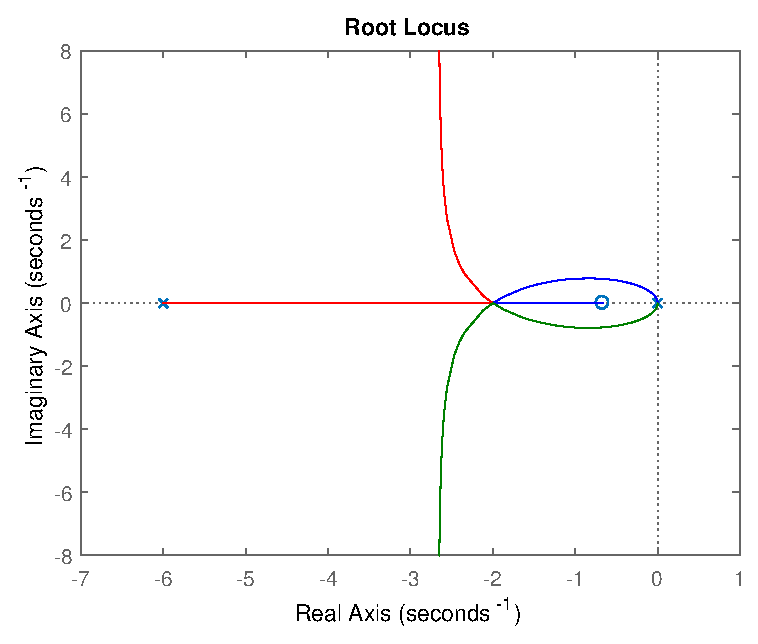
\includegraphics [width=7in]{MidtermPrep_05.eps}



\end{document}
    
